\section{Overview of System \sys{}}
\label{sec:overv}

\subsection{Problem Formulation}
% {user, blog, user-blog} => model
% query (a user u, a blog b that is created or forwarded by u's friend)
% returns: Y/N u shall forward b

\par We consider the \retg{} behavior of users in social media.
%For simplicity, with a given user, we assume that microblogs created or \retd{} by his/her followees cover the overall candidates, from which the said user may \ret{}.
For simplicity, assuming the microblogs that a user can \ret{} come from those owned by his/her followees.

%All our results could straightforwardly generalize to alternative candidate scopes.
%e.g., the like/unlike behavior against the candidate of remarking [double check the network language; register a Facebook]
%e.g., positive comments in the overall comments

\begin{definition}
\label{def:blog}
A microblog $M_b = (O, T, M, flag)$ has its owner $O$ (a.k.a. user in this paper) to whom $M_b$ belongs (either \twd{} or \retd{}), the generated time $T$ of $M_b$, the message context $M$, and $flag$ denoting $M_b$ is \retd{} or originally \tw{} by $O$. Here we use 1 and 0 to denote \retd{} and  \tw{}, respectively.
\end{definition}

\begin{comment}
\begin{definition}
A blog $B = (O, T, M, C)$ consists of the owner $O$ to whom $B$ belongs (either created or \retd{}), the timestamp $T$ showing when $B$ is generated, the blog message $M$ and a set of counters $C_s(B) = \{\#comment,\ \#like,\ \#\ret{}\}$ regarding the number of being commented, liked, and \retd{}.
\end{definition}
\end{comment}

\begin{definition}
\label{def:user}
Given a user $u$, we adopt $B_u$, $R_u$ and $E_u$ to represent her/his microblogs $B_u$, followers $R_u$ and followees $E_u$,  respectively, in which a follower/followee is a user.
\end{definition}

%The mapping between blog $B$ and user $U$ is a bilateral operation, i.e., $U = O(B)$ and $B \in B_s(U)$, through ID(s) of user and blog respectively.
Note that $M_b.O$ is a user, and $B_u$ is a set of microblogs.


Providing a set of users $\mathbb{U}$ and their associated microblogs $\mathbb{B}$, system \sys{} builds a \retg{} model for each group of  $\mathbb{U}$, such that given a microblog $b$ and a follower $f$ of its onwer $b.O$, i.e., $f \in R_{b.O}$, 1 or 0 is returned regarding whether $f$ \ret{s} $b$ or not.

\begin{figure}[tb!]
\centering
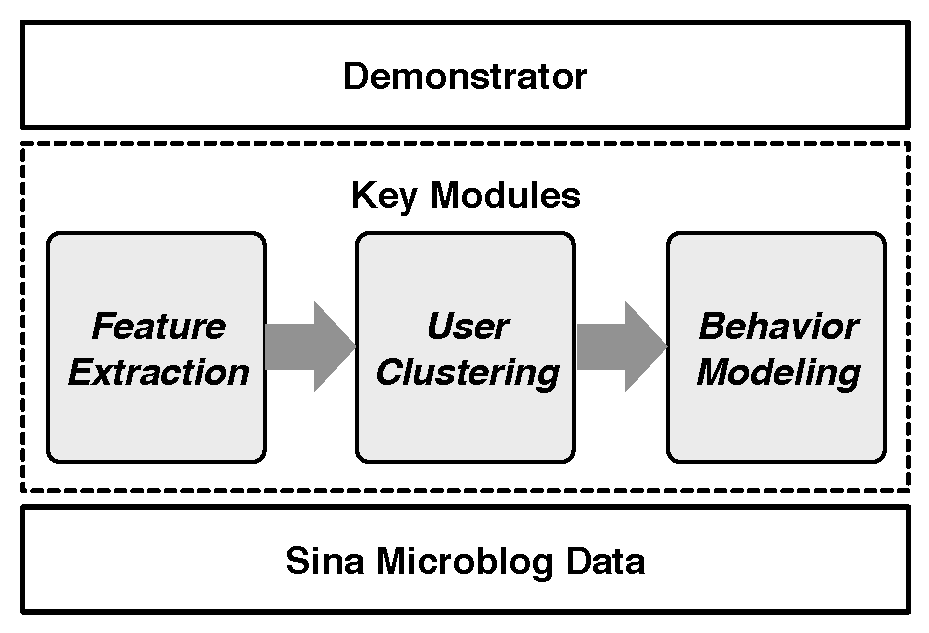
\includegraphics[width=.6\linewidth]{figures/architecture.eps}
%\vspace{-1ex}
\caption{\sys{} Architecture}
\label{fig:framework}
\vspace{-2ex}
\end{figure}


%This section shall look into the principle of each component in Processing Runtime subsystem, putting forth a full-fledged system.

\subsection{\sys{} Framework}
System \sys{} is designed from the ground up as a system for modeling users' \retg{} behavior in social media, and
Figure \ref{fig:framework} shows the architectural components of \sys{}. %, mainly comprising Sina Microblog Data, Key Modules and Profile Demonstrator.





% #like and #comment are saved; could generalize \sys{} to model the liking behavior (among commented blogs)
\begin{comment}
\begin{figure}[!htb]
\centering
\includegraphics[width=.99\linewidth]{figures/microblog}
\caption{Blog Data in \sys{}}
\label{fig:blog}
\end{figure}
\end{comment}

\begin{comment}
\begin{figure}[!htb]
\centering
\includegraphics[width=.99\linewidth]{figures/user}
\caption{User Data in \sys{}}
\label{fig:user}
\end{figure}
\end{comment}





\stitle{Sina Microblog Data.} It is the data crawled to be processed by \sys{}, i.e., data of microblogs and users.

\stitle{Key Modules.}
\sys{} consists of three key modules.
%\begin{enumerate}

	\stab(1)  Feature Extraction: By coalescing the microblog data, each user is depicted by a bunch of features, which are grouped into three categories. They are features of \textit{Basics} (e.g., the number of followers and followees), \textit{Behavior} (e.g., the frequency and the popular slots of \retg{}) and \textit{Interest} (e.g., long and short term interests, as well as explicit and implicit interests). These features are extracted from the stored  Sina Weibo data by Feature Extraction module, and serve as the input of the User Clustering module.
	
	\stab(2)  User Clustering: Providing the user-based features, User Clustering takes charge of the clustering task such that each user falls into a proper group.
	
	\stab(3)  Behavior Modeling: For each group obtained by User Clustering, Behavior Modeling builds a  model by employing both positive and negative samples (i.e., microblogs labeled with \retd{} and not \retd{}), on which the user \retg{} behaviors are also tested.
%\end{enumerate}
	
\stitle{Demonstrator.} At the top layer of \sys{}, it is the Demonstrator for visualizing all aspects of the system, e.g., profiling of user groups.
%For the time being, Profile Demonstrator presents \tbc{}.


The distinctive feature of System  \sys{} models user \retg{} behaviors over groups instead of a single model for all the users \cite{IEEEexample:conf/wsdm/FengW13,IEEEexample:conf/ijcai/ZhangLTCL13}.

